\section{Diccionario de actores}
A continuación se describen los diferentes tipos de usuarios que se encuentran dentro del funcionamiento del sistema.\\

\begin{itemize}
\item Usuario cliente: Se refiere a todo cliente o consumidor de una tienda departamental o comercio el cual interactuará directamente con la aplicación móvil difusora de productos.
\item Usuario vendedor: Se refiere a los encargados de proporcionar información y atender presencialmente a los clientes de un establecimiento.
\item Usuario administrador: Se define como usuario administrador a aquellas personas encargadas de seleccionar los productos que se encuentran con promociones y a su vez divulgarlos por medio de un folleto informativo.

\item Usuario desarrollador: Se define a este usuario como los integrantes del equipo Sapphire, encargado de ejecutar el generador de registros artificiales y de evaluar las pruebas dentro del guión de pruebas.
\end{itemize}
\section{Diagrama de casos de uso general}
La siguiente figura \ref{image:casosdeusogenerales}, muestra el diagrama de casos de uso en el cual se observa de forma general las acciones que tendrán permitidas los actores previamente definidos.

\FloatBarrier
\begin{figure}[htbp!]
		\centering
			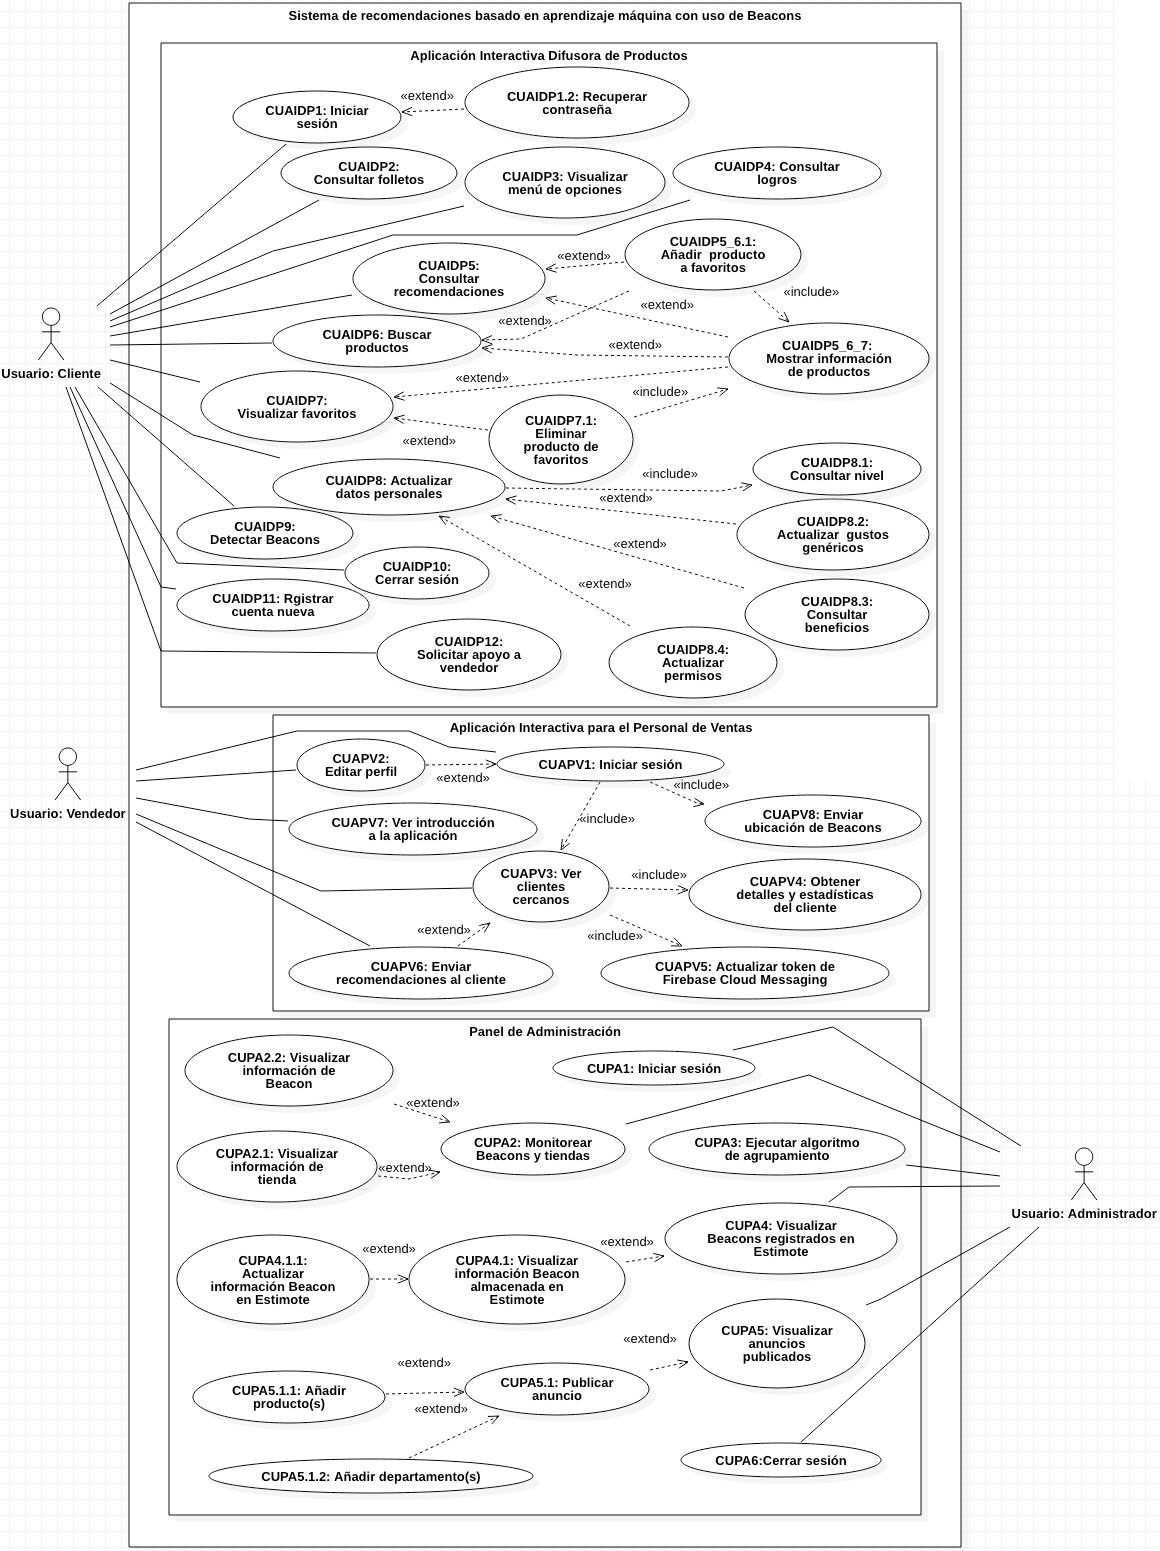
\includegraphics[width=1 \textwidth]{imagenes/casosGenerales1}
		\caption{Diagrama de casos de uso general.}
		\label{image:casosdeusogenerales}
\end{figure}
\FloatBarrier

\section{Requerimientos Funcionales (RF)}
A continuación se muestran del cuadro \ref{table:requerimientosfGRA} al cuadro \ref{table:requerimientosfMGPYPDR}, los requerimientos funcionales que están compuestos tanto por las aplicaciones móviles como por los servidores y los cuales consisten en las funcionalidades requeridas por cada uno de los módulos mencionados con el fin de que el proyecto en su totalidad funcione adecuadamente.\\

\title{\textbf{Requerimientos Funcionales del Generador de Registros Artificiales (RFGRA)}}
\hypertarget{RFGRA}{}
\begin{FRequirements}
\FRitem{RFGRA1}{Menú principal}{Debe existir un menú principal que le permita al usuario desarrollador seleccionar el tipo de acción a realizar.}

\FRitem{RFGRA2}{Generar persona}{Se debe permitir crear automáticamente personas ficticias y registrarlas en el repositorio del sistema.}

\FRitem{RFGRA3}{Generar dirección}{El módulo generador de registros artificiales debe permitir crear automáticamente direcciones ficticias que existan en dentro del territorio de la República Mexicana para posteriormente registrarlas en el repositorio de datos.}

\FRitem{RFGRA4}{Generar tienda}{El módulo generador de registros artificiales permitirá insertar en el repositorio de datos tiendas ficticias.}

\FRitem{RFGRA5}{Generar departamento}{Se debe permitir generar automáticamente departamento asociados a una tienda.}

\FRitem{RFGRA6}{Generar productos}{Dentro del módulo generador de registros artificiales debe exister la opción para crear automáticamente productos ficticios e insertarlos en el repositorio de datos del sistema.}

\FRitem{RFGRA7}{Generar imágenes pertenecientes a productos}{El módulo debe contener la funcionalidad para crear imágenes ficticias de productos que serán agregadas al repositorio de datos con el fin de hacer los registros persistentes.}

\FRitem{RFGRA8}{Asignar imágenes a productos}{El módulo debe poder asignar automáticamente imágenes a productos que estén registrados en el repositorio de datos y así mismo, almacenarlas en dicho repositorio.}


\FRitem{RFGRA9}{Generar empleados}{Se debe permitir generar automáticamente y almacenar en el repositorio de datos, empleados que trabajen en alguna tienda registrada en el sistema con respecto a las personas que existen en el repositorio de datos.}

\FRitem{RFGRA10}{Generar clientes}{Debe existir la posibilidad de generar clientes ficticios con respecto a las personas ya registradas en el repositorio de datos y a su vez, registrar a dichos clientes en el repositorio.}

\FRitem{RFGRA11}{Asignar productos favoritos a clientes}{El módulo en cuestión debe permitir generar registros ficticios de productos añadidos a favoritos por un usuario, mismos que se almacenarán en el repositorio de datos.}

\FRitem{RFGRA12}{Generar compras a clientes}{El Generador de Registros Artificiales debe permitir generar compras ficticias de productos a un usuario cliente, mismos que se almacenarán en el repositorio de datos.}

\FRitem{RFGRA13}{Generar asignar logros y nivel a clientes}{Se debe permitir generar logros y asignar un nivel dependiendo de los movimientos que haya tenido el usuario cliente en el sistema}
\caption{Requerimientos Funcionales del Generador de Registros Artificiales.}
\label{table:requerimientosfGRA}
\end{FRequirements}




\title{\textbf{Requerimientos Funcionales de la Aplicación Interactiva Difusora de Productos (RFAIDP)}}
\hypertarget{RFAIDP}{}
\begin{FRequirements}
\FRitem{RFAIDP1}{Iniciar sesión}{\hypertarget{RFAIDP1}{}La aplicación controlará el acceso del cliente a esta mediante el inicio de sesión con la API de Facebook.
}

\FRitem{RFAIDP2}{Consultar folletos}{\hypertarget{RFAIDP2}{}La aplicación mostrará al cliente en la pantalla principal, después de iniciar sesión, los productos que se encuentran actualmente con descuento o las promociones actuales en las tiendas. Dichas promociones serán generados respecto a las diferentes celebraciones del mes (Día de la madre, Navidad, etc.) o por un motivo en particular como su cumpleaños.
}

\FRitem{RFAIDP3}{Visualizar menú de opciones}{El cliente podrá visualizar dentro de la aplicación móvil las diferentes opciones que este le ofrece mediante la apertura de un menú lateral. Entre dichas opciones se encuentran las siguientes:
\hypertarget{RFAIDP3}{}
\begin{itemize}
\item Inicio,
\item Logros,
\item Favoritos,
\item Recomendaciones,
\item Búsqueda de productos,
\item Ver Perfil,
\item Cerrar Sesión.
\end{itemize}
Cada una de dichas opciones deberá direccionar al usuario a su pantalla correspondiente.
}

\FRitem{RFAIDP4}{Consultar logros}{\hypertarget{RFAIDP4}{}Será la pantalla a la cual direccione la opción ``Logros'' del menú lateral. Un logro será por ejemplo los siguientes:
\begin{itemize}
\item Comprar con tarjeta de crédito.
\item Comprar un producto en una tienda más de 7 veces.
\item Realizar una compra igual o mayor a \$3000.00.
\end{itemize} 
Entre otros que serán posteriormente especificados por cada tienda en particular y por los cuales, dicho usuario obtendrá una recompensa por su logro que pueden ser descuentos en sus próximas visitas o meses sin intereses entre otros.
}

\FRitem{RFAIDP5}{Añadir producto a favoritos}{\hypertarget{RFAIDP5}{}El cliente tendrá la opción de almacenar aquellos productos recomendados y/o encontrados que resulten ser de su interés cuando los busque en la sección del menú ``Búsqueda de productos''.
}

\FRitem{RFAIDP6}{Visualizar favoritos}{\hypertarget{RFAIDP6}{}El cliente tendrá la oportunidad de visualizar todos los productos que ha añadido previamente a la sección de ``Favoritos''.
}

\FRitem{RFAIDP7}{Consultar recomendaciones}{\hypertarget{RFAIDP7}{}El cliente podrá observar al presionar la opción del menú lateral ``Recomendaciones'', un listado de productos recomendados específicamente para él, mismos que han sido generadas mediante el algoritmo de recomendación basado en filtrado colaborativo.
}

\FRitem{RFAIDP8}{Buscar productos}{\hypertarget{RFAIDP8}{}El cliente tendrá una sección llamada ``Búsqueda de productos'' en el menú lateral, en la cuál tendrá la posibilidad de buscar por nombre de producto, cualquier producto que requiera o desee.
}

\FRitem{RFAIDP9}{Actualizar datos personales}{\hypertarget{RFAIDP9}{}El cliente podrá consultar sus datos personales en la sección ``Ver Perfil'', misma que se ha obtenido por default desde su cuenta de Facebook, dicha información involucra su nombre, foto de perfil y correo electrónico. Sin embargo, deberá acompletar su información personal con el fin de categorizarlo correctamente dentro de un grupo con características similares, para ello, deberá incluir:  
\begin{itemize}
\item Sexo,
\item Estado civil,
\item Fecha de nacimiento.
\end{itemize}
Esta sección aparecerá en la sección ``Ver Perfil'' del menú lateral.
}

\FRitem{RFAIDP10}{Consultar nivel}{\hypertarget{RFAIDP10}{}Según los logros que el cliente vaya obteniendo, su nivel irá incrementando dentro de la aplicación, mismo que podrá consultar en su perfil.
}

\FRitem{RFAIDP11}{Actualizar gustos genéricos}{\hypertarget{RFAIDP11}{}Para proporcionar al usuario recomendaciones más acertadas de acuerdo a sus gustos y preferencias, deberá seleccionar de una lista aquellos que se asemejen más a los suyos, entre estos están:
\begin{itemize}
\item Hogar,
\item Computadoras,
\item Celulares y tablets,
\item TV y video,
\item Cámaras,
\item Audio,
\item Videojuegos,
\item Drones y radio control,
\item Wearables,
\item Instrumentos musicales,
\item Autos, motos y GPS,
\item Hogar inteligente,
\item Salud y belleza,
\item Películas y series.
\end{itemize}
Esta sección aparecerá en la sección ``Ver Perfil'' del menú lateral, dentro de una pestaña en la parte superior de esta pantalla.
}

\FRitem{RFAIDP12}{Consultar beneficios}{\hypertarget{RFAIDP12}{}Según el nivel en el que se encuentre el cliente a partir de sus compras, podrá obtener y consultar diferentes beneficios tales como envíos gratis y descuentos en particulares. Esta sección aparecerá en la sección ``Ver Perfil'' del menú lateral, dentro de una pestaña en la parte superior de esta pantalla.
}

\FRitem{RFAIDP13}{Actualizar permisos}{\hypertarget{RFAIDP13}{}El cliente tendrá la posibilidad de permitir mostrar a los vendedores parte de su información personal como lo es:
\begin{itemize}
\item Edad
\item Estado civil
\item Número de hijos
\item Productos seleccionados como favoritos
\item Compras realizadas recientemente
\end{itemize}
Y de igual manera, permitir a los vendedores acercarse a ellos para ofrecerles distintos productos que puedan ser de su interés. Deberá marcar la casilla correspondiente a los permisos que desee en la sección de ``Ver Perfil'', en la pestaña de ``Permisos''.
}

\FRitem{RFAIDP14}{Detectar Beacons}{\hypertarget{RFAIDP14}{}El dispositivo móvil del cliente requiere contar con un BLE que sea capaz de detectar los Beacons que se encontrarán en ciertas zonas de las tiendas. Al captar la señal de alguno de ellos, obtendrá una pequeña alerta con información sobre el piso al que acaba de ingresar, por ejemplo.
}

\FRitem{RFAIDP15}{Cerrar sesión}{\hypertarget{RFAIDP15}{}El cliente podrá cerrar su sesión de Facebook con la cual ingresó a la aplicación móvil con la finalidad de ingresar con cuentas alternativas.
}


\FRitem{RFAIDP16}{Registrar cuenta nueva}{\hypertarget{RFAIDP16}{}El cliente podrá crear una cuenta nueva a partir del ingreso de datos solicitados en el formulario como:
\begin{itemize}
\item Nombre,
\item Apellido paterno,
\item Apellido materno,
\item Correo electrónico,
\item Contraseña,
\item Estado civil,
\item Fecha de nacimiento.
\end{itemize}
}


\FRitem{RFAIDP17}{Recuperar contraseña}{\hypertarget{RFAIDP17}{}En caso de olvidar su contraseña, el cliente podrá solicitar que le sea enviada al correo electrónico que introduzca.
}

\FRitem{RFAIDP18}{Eliminar producto de favoritos}{\hypertarget{RFAIDP18}{}En caso de que el cliente haya añadido un producto a la sección de favoritos y no lo desee más, tendrá la opción de eliminar dicho producto de esta sección al presionar sobre algún producto en particular.
}

\FRitem{RFAIDP19}{Mostrar información de productos}{\hypertarget{RFAIDP19}{}Si el cliente presiona sobre un artículo en particular se desplegará una nueva ventana con la información de dicho producto e imágenes de este.
}

\FRitem{RFAIDP20}{Solicitar apoyo a vendedor}{Si el cliente presiona sobre la opción ``Solicitar apoyo'' localizada en el menú de opciones, un vendedor podrá acercarse a él para proveer la ayuda que él requiera.
}

\caption{Requerimientos Funcionales de la Aplicación Interactiva Difusora de Productos.}

\end{FRequirements}






\title{\textbf{Requerimientos Funcionales de la Aplicación Interactiva para el Personal de Ventas (RFAIPV)}}
\begin{FRequirements}
\hypertarget{RFAPV}{}
\FRitem{RFAPV1}{Iniciar sesión}{La aplicación controlará el acceso del usuario vendedor por medio del nombre de usuario del vendedor  y su respectiva contraseña.
}

\FRitem{RFAPV2}{Enviar de ubicación de beacons}{
La aplicación deberá detectar y enviar al Sistema de Gestión, Procesamiento y Proveedor de Datos Retail las ubicaciones de los diferentes beacons registrados alrededor del centro comercial.
}

\FRitem{RFAPV3}{Editar perfil del vendedor}{
La aplicación permitirá al usuario vendedor editar sus datos personales básicos (nombre, apellidos, email y contraseña).
}

\FRitem{RFAPV4}{Ver clientes cercanos}{
La aplicación permitirá al usuario vendedor visualizar un listado de los clientes cercanos dentro de un comercio o establecimiento con la finalidad de brindarle apoyo personalizado en caso de ser requerido por un usuario cliente o enviar recomendaciones personalizadas del departamento en el que se encuentre el cliente.
}

\FRitem{RFAIPV5}{Obtener detalles y estadísticas de un cliente}{
La aplicación permitirá al vendedor visualizar detalles de un cliente: sexo, edad, número de hijos, beneficios por su nivel, 5 productos favoritos; así como estadísticas de compra: total de compras realizadas en los últimos 6 meses y las categorías de productos más comprados. Estos datos se mostrarán únicamente si el cliente otorga el permiso de visualización para cada uno de ellos.
}

\FRitem{RFAIPV6}{Enviar recomendaciones a clientes}{
La aplicación permitirá al vendedor enviar recomendaciones de productos del departamento en el que los clientes se encuentren.
}

\FRitem{RFAIPV7}{Actualizar token de Firebase Cloud Messaging (FCM)}{
La aplicación permitirá actualizar el token de FCM para subscribirse a las notificaciones de cada uno de los departamentos a los que el vendedor se dirija, es decir, cada que el vendedor cambie de departamento de igual forma lo hará el token.
}
\caption{Requerimientos Funcionales de la Aplicación Interactiva para el Personal de Ventas.}
\end{FRequirements}

\title{\textbf{Requerimientos Funcionales del Panel de Administración (RFPA)}}
\hypertarget{RFPA}{}
\begin{FRequirements}
\FRitem{RFPA1}{Iniciar sesión}{El panel de administración controlará el acceso de un usuario administrador al panel de administración por medio de un nombre de usuario y su respectiva contraseña.
}

\FRitem{RFPA2}{Monitorear Beacons y tiendas}{
El panel de administración deberá tener un apartado donde se permita plasmar en un mapa la geolocalización de los Beacon y tiendas que se encuentran disponibles por toda la República Mexicana. Así mismo, se mostrará la información básica de dichos Beacons como su id, nombre, batería, departamento al que pertenece; de igual manera, para las tiendas departamentales se mostrará su nombre y su dirección.
}

\FRitem{RFPA3}{Visualizar información de anuncios publicados}{
El panel de administración deberá tener un apartado donde se permita visualizar la información de los anuncios publicados en el sistema. Por otra parte, se debe permitir registrar nuevos anuncios con sus respectivos productos y departamentos asociados.}

\FRitem{RFPA4}{Visualizar información de Beacons}{
El panel de administración deberá contar con  un apartado donde se permita ver la información de los Beacon registrados en el sistema. Por otra parte, se debe permitir modificar algunos campos de cada Beacon.}

\FRitem{RFPA5}{Ejecutar algoritmo de agrupamiento}{
El panel de administración deberá contar con  un apartado en el cuál se permita actualizar los grupos de personas formados anteriormente, además de mostrar la información más relevante de cada grupo.}

\caption{Requerimientos Funcionales del Panel de Administración.}
\end{FRequirements}

\title{\textbf{Requerimientos Funcionales del Sistema de Gestión, Procesamiento y Proveedor de datos de Retail (RFGPPR)}}
\hypertarget{RFSGPyPDR}{}

\FloatBarrier
\begin{FRequirements}

\FRitem{RFGPPR1}{Conectar con módulos basados en aprendizaje máquina}{
El SGPPDR (Sistema de Gestión, Procesamiento y Proveedor de Datos Retail) se encargará de conectarse con los dos módulos basados en aprendizaje máquina, con el fin de formular una serie de recomendaciones de productos a partir de los ya comprados previamente por el usuario y los comprados por usuarios cliente con características similares a las del usuario cliente en cuestión.
}

\FRitem{RFGPPR2}{Generar módulo clustering}{El módulo interno llamado módulo de análisis de datos podrá conformar diferentes grupos de usuarios cliente con base en los gustos y características de éstos para posteriormente almacenar dichas agrupaciones en el repositorio de datos. 
}

\FRitem{RFGPPR3}{Generar módulo de recomendaciones basado en filtrado colaborativo}{
El módulo tomará los registros almacenados previamente por el módulo de clustering y realizará las recomendaciones basado en las compras de los usuarios cliente pertenecientes (también llamado vecindario) al mismo grupo en el que ellos se encuentran.
}

\FRitem{RFGPPR4}{Ejecutar algoritmo de agrupamiento}{
Debe ser posible ejecutar el algoritmo de agrupamiento sobre los usuarios ya existentes y/o usuarios nuevos.
}

\FRitem{RFGPPR5}{Obtener clusters y características}{
El sistema debe tener la funcionalidad necesaria para proveer los clusters y sus características principales.
}
%----------PANEL BEGIN-------%
\FRitem{RFGPPR6}{Registrar folletos}{
El SGPPDR debe tener la funcionalidad necesaria para poder hacer el registro de folletos nuevos al sistema.
}
\FRitem{RFGPPR7}{Obtener folletos: Administrador}{
El SGPPDR debe mostrar los folletos registrados en el sistema.
}
\FRitem{RFGPPR8}{Proveer Beacons registrados}{
Debe existir la funcionalidad para proveer los Beacons registrados en sistema a la aplicación cliente Panel de Administración.
}
\FRitem{RFGPPR9}{Proveer establecimientos registrados}{
Debe existir la funcionalidad para proveer los establecimientos registrados en el repositorio de datos a la aplicación cliente Panel de Administración.
}
\FRitem{RFGPPR10}{Proveer departamentos dentro de tienda}{
El sistema debe tener la funcionalidad necesaria para proveer los departamentos asignados a una tienda o establecimiento.
}
\FRitem{RFGPPR11}{Insertar/Actualizar Beacons del sistema}{
Debe existir la opción para insertar nuevos Beacons al sistema, por otra parte, si un Beacon ya está registrado se debe poder actualizar su posición actual. 
}

\FRitem{RFGPPR12}{Obtener atributos clave-valor de Beacons}{
Debe ser posible obtener los atributos clave-valor (attachments) de los Beacons registrados desde Estimote Cloud para con ellos se puedan crear las zonas de proximidad.
}

\FRitem{RFGPPR13}{Proveer token de autenticación: Administrador}{
El sistema recibirá los datos de autenticación de un usuario administrador para posteriormente devolver un token de autenticación al panel de administración.
}
%----------PANEL END-------%
%----------AIPV BEGIN-------%

\FRitem{RFGPPR14}{Proveer token de autenticación: Vendedor}{
El sistema recibirá los datos de autenticación de un usuario vendedor para posteriormente devolver un token de autenticación a la aplicación interactiva para el personal de ventas.
}

\FRitem{RFGPPR15}{Actualizar token de Firebase Cloud Messaging (FCM) para vendedor}{
Un usuario vendedor debe poder actualizar su token de Firebase Cloud Messaging para las notificaciones push.
}
\FRitem{RFGPPR16}{Actualizar datos básicos del perfil del vendedor}{
Debe existir la posibilidad de modificar los datos personales o profesionales de los empleados registrados en el sistema.
}

\FRitem{RFGPPR17}{Obtener clientes cercanos en departamento}{
Cuando un usuario cliente se encuentre dentro de un departamento asignado a un Beacon el usuario vendedor debe ser capaz de obtener la información de todos los usuarios cliente dentro del área de proximidad del Beacon.
}
\FRitem{RFGPPR18}{Obtener detalles y estadísticas de cliente}{
El sistema debe devolver al vendedor cuando lo solicite, los detalles y estadísticas a las que el cliente haya otorgado permisos.
}
\FRitem{RFGPPR19}{Obtener recomendaciones por departamento}{
El sistema debe permitirle a un vendedor ver las recomendaciones de un cliente cuando se encuentre dentro del mismo departamento que el usuario vendedor.
}
\FRitem{RFGPPR20}{Enviar recomendaciones a cliente}{
El sistema debe permitirle a un vendedor enviar una recomendación de un producto a un cliente por medio de una notificación push usando FCM.
}

\FRitem{RFGPPR21}{Insertar/Actualizar Beacons de desde la AIPV}{
El sistema debe permitirle a un vendedor actualizar la ubicación de un Beacon para mantener el control de los mismos.
}
%----------AIDP BEGIN-------%

\FRitem{RFGPPR22}{Registrar clientes}{
Debe existir la funcionalidad necesaria para poder hacer el registro de clientes nuevos al sistema.
}
\FRitem{RFGPPR23}{Obtener información del cliente}{
Un usuario cliente debe tener la posibilidad de obtener su información personal en cualquier momento.
}
\FRitem{RFGPPR24}{Proveer de productos}{
El SGPPDR recibirá peticiones de productos por parte de ambas aplicaciones móviles para posteriormente devolver los productos incidentes a dicha petición.
}
\FRitem{RFGPPR25}{Proveer de folletos}{
El módulo deberá proveer a la aplicación interactiva difusora de productos los folletos relevantes en el momento requerido.
}
\FRitem{RFGPPR26}{Agregar producto a favoritos}{
El módulo debe permitir a un cliente agregar un producto a sus productos favoritos.
}
\FRitem{RFGPPR27}{Actualizar token de Firebase Cloud Messaging para cliente}{
Un usuario cliente debe poder actualizar su token de Firebase Cloud Messaging para las notificaciones push.
}
\FRitem{RFGPPR28}{Publicar ubicación de cliente en Kafka}{
Cuando un usuario cliente entre a una zona de proximidad asignada a un Beacon su posición se debe publicar en el sistema.
}
\FRitem{RFGPPR29}{Obtener recomendaciones globales}{
El sistema debe permitirle a un usuario cliente ver sus recomendaciones de todos los productos registrados en el repositorio de datos.
}
%----------AIDP END-------%

\caption{Requerimientos Funcionales del Sistema de Gestión, Procesamiento y Proveedor de datos de Retail.}
\label{table:requerimientosfMGPYPDR}
\end{FRequirements}



\section{Requerimientos No Funcionales (RNF)}
Los requerimientos no funcionales corresponden a aquellos criterios que son necesarios para medir el desempeño del sistema tanto internamente como con la interacción de este con el usuario. En la parte inferior se muestra en el cuadro \ref{table:requerimientosNoFuncionales} los requerimientos no funcionales del sistema. 
\begin{NFRequieriments}
\NFRitem{RNF1}{Eficiencia}{
\begin{itemize}
\item Los datos modificados en el repositorio de datos deben ser actualizados para todos los usuarios que acceden al sistema en cuanto actualicen o cambien de pantalla.
\end{itemize}
}
\NFRitem{RNF2}{Usabilidad}{
\begin{itemize}
\item El sistema debe contar con manuales de usuario estructurados adecuadamente.
\item El sistema debe proporcionar mensajes de error que sean informativos y orientados a usuario final.
\item El sistema debe contar con un módulo de ayuda en línea.
\item La aplicación Web debe poseer un diseño “responsive” a fin de garantizar la adecuada visualización en múltiples computadores personales, dispositivos tableta y teléfonos inteligentes.
\end{itemize}

}

\NFRitem{RNF4}{Portabilidad}{
\begin{itemize}
\item Las aplicaciones móviles funcionarán únicamente en la plataforma Android. 
\item La aplicación móvil debe funcionar a partir de la versión 4.3 de Android.
\item El panel de administración debe funcionar en las plataformas Windows, Linux y MacOs.
\item El panel de administración será implementado para navegadores Web únicamente con HTML5 y Javascript.
\end{itemize}
}
%
%\NFRitem{RNF5}{Privacidad de datos personales}{
%\begin{itemize}
%\item Para protección del cliente, el sistema no debe mostrar datos personales a los empleados, únicamente un nickname o pseudónimo y una foto de perfil (que no necesariamente debe ser una foto del mismo).
%\end{itemize}

%}

\NFRitem{RNF5}{Diseño responsivo}{
\begin{itemize}
\item EL Panel de Administración debe poseer un diseño “responsive” a fin de garantizar la adecuada visualización en múltiples computadores personales y dispositivos tableta.
\end{itemize}
}

\caption{Requerimientos No Funcionales del sistema.}
\label{table:requerimientosNoFuncionales}
\end{NFRequieriments}
\newpage
